The mission of the International Linear Collider (ILC) is to explore the fundamental composition of nature, i.e. the material and energy constituting the universe, by observing reactions among fundamental particles at the extremely high energy attainable in the superconducting linear collider.
 
\subsubsection{Design}

The electron source for the ILC will use 2 $ns$ laser light pulses to eject electrons from a photocathode, a technique allowing for up to 90\% of the electrons to be polarised; the electrons then will be accelerated to 5 GeV in a 370 meter linac stage. Synchrotron radiation from high energy electrons will produce electron-positron pairs on a titanium-alloy target, with 30\% polarisation; the positrons from these collisions will be collected and accelerated to 5 GeV in a separate linac.
To compact the 5 GeV electron and positron bunches to a sufficiently small size to be usefully collided, they will circulate for 0.1\textendash 0.2 seconds in a pair of damping rings, 3.24 km in circumference, in which they will be reduced in size to 6 mm in length and a vertical and horizontal emittance of 2 pm and 0.6 nm, respectively.
From the damping rings the particle bunches will be sent to the superconducting radio frequency main linacs, each 11 km long, where they will be accelerated to 250 GeV. At this energy each beam will have an average power of about 5.3 MW. Five bunch trains will be produced and accelerated per second.
To maintain a sufficient luminosity to produce results in a reasonable time frame after acceleration the bunches will be focused to a few nanometers in height and a few hundred nanometers in width. The focused bunches then will be collided inside one of two large particle detectors.

\begin{figure}[!htb]
\centering
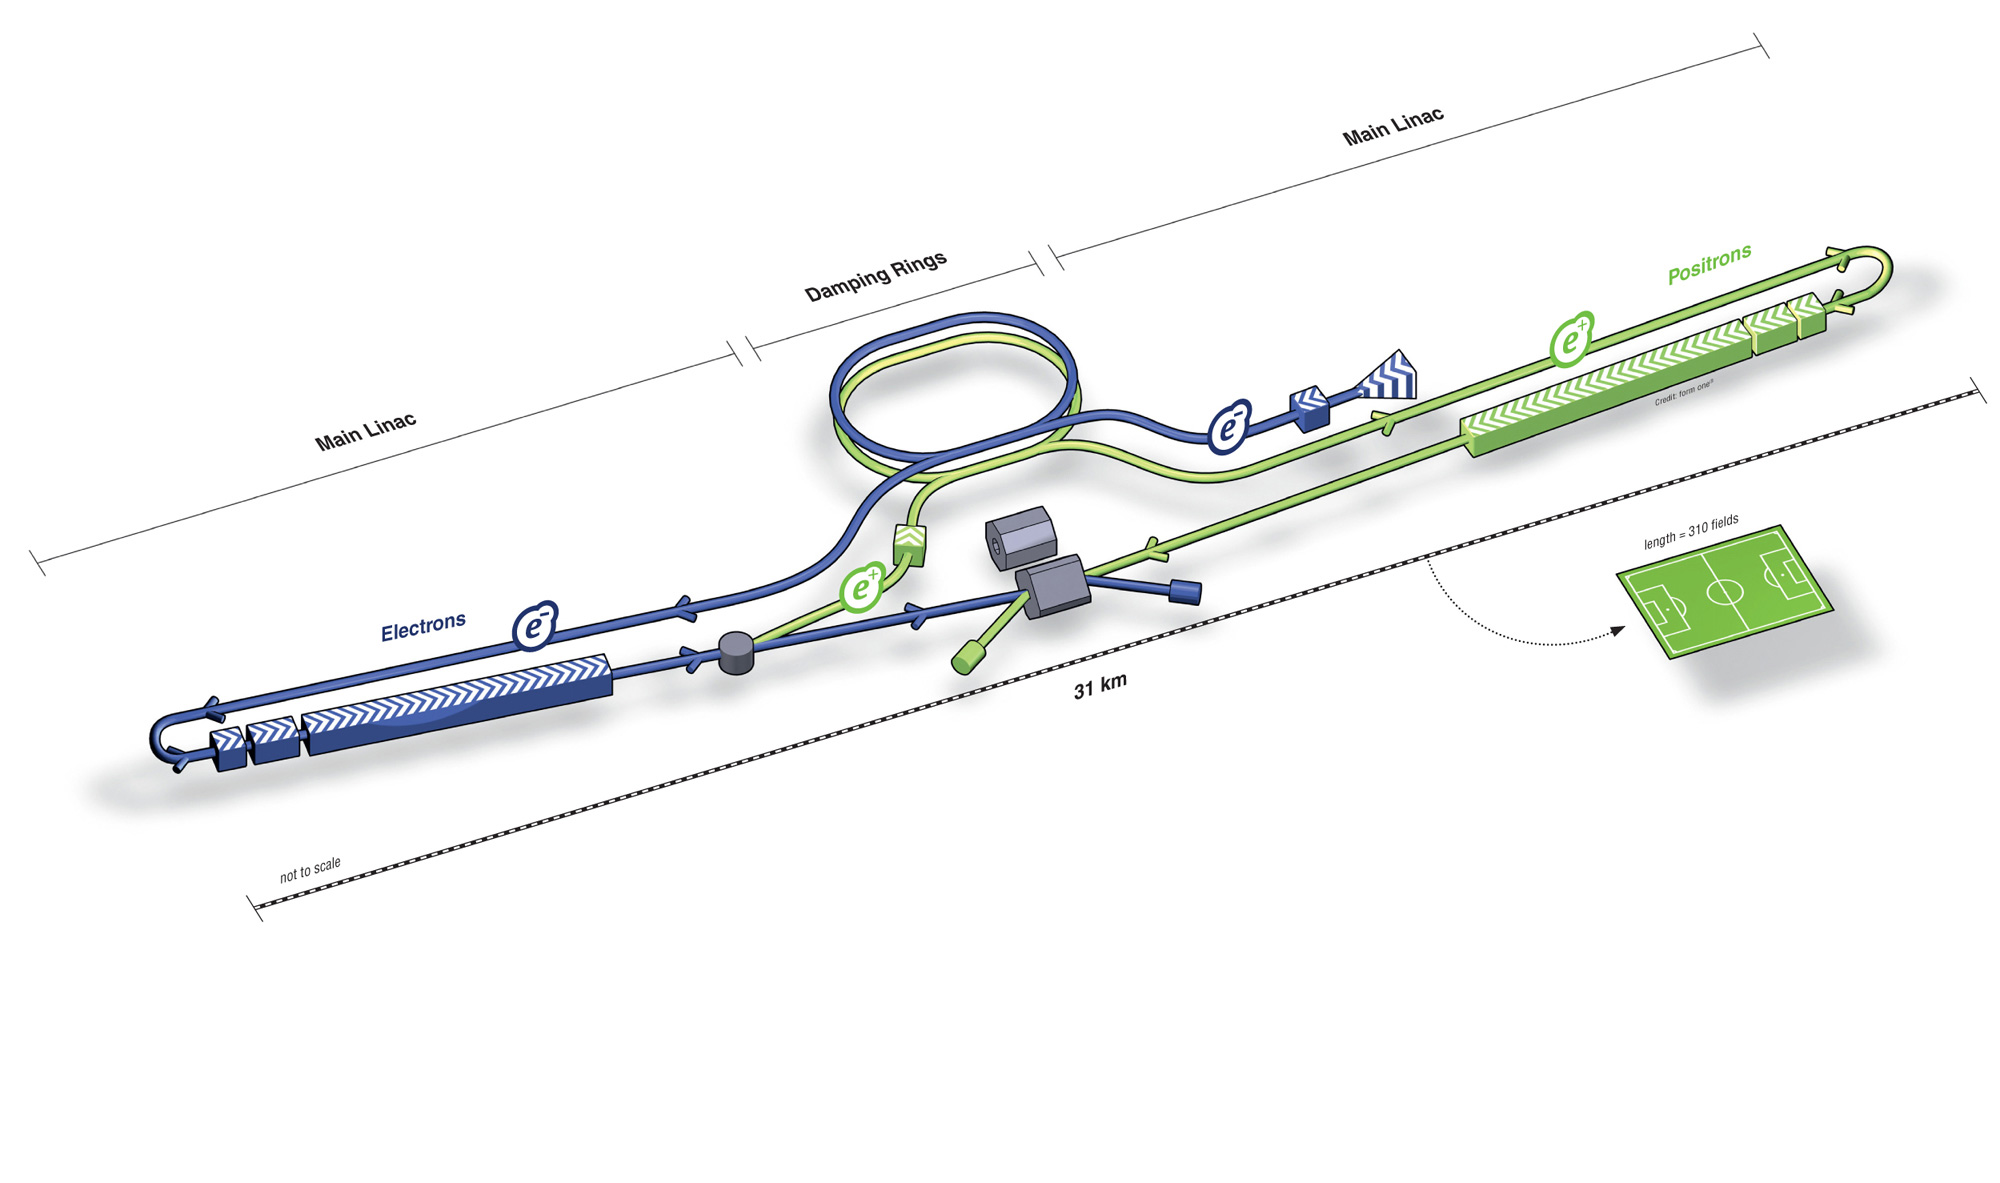
\includegraphics[width=1\textwidth,natwidth=2000,natheight=1183]{ILC_Diagram.jpg}
\caption{ILC Concept Schematic \cite{ILC:Images}}
\end{figure}

\subsubsection{Goals \cite{ILC:TechnicalDesignReport}}

\begin{enumerate}
  \item Measure the mass, spin, and interaction strengths of the Higgs boson.
  \item If discovered, measure the number, size, and shape of any TeV-­‐scale extra     dimensions.                                         
  \item Investigate the lightest supersymmetric particles, possible candidates for dark matter.
\end{enumerate}

\subsubsection{Spin-offs}

There are two types of spin-offs. The first is a reappropriation of innovative
technology originally developed for scientific research. A remarkable case in particle
accelerators research, for example, is the spilling over of high performance
electromagnetic steel specifically improved and fabricated as the iron core for accelerator magnets. The electric machinery industry has combined the high performance electromagnetic steel with substantive progress in electromagnetic field analysis software to manufacture a variety of electric machinery with lower and lower power loss rates. 

Another example is a spilling over of newly developed systems/subsystems themselves and/or common technology thereof to related industry sectors. A conspicuous illustration of this case is seen in the expanding applications of the electron linac, which was initially developed solely for nuclear and high energy physics research, to the medical and non-destructive inspection industries. Another well-known example is the growing application of superconducting magnets, having been greatly improved as an outcome of its successive adoption in particle accelerators, not only to industrial sectors such as medical therapy, material research, and power generation/transmission, but also to a magnetic levitation, ultra-high speed public transportation system. \cite{ILC:SpinOffReport}
 
\subsubsection{Feasibility}

%todo not a lot of analysis here, just facts and figures
The 500 GeV ILC technical design presented in the ILC Technical Design Report (TDR) has been developed based on an extensive R\&D program. The R\&D has
successfully demonstrated the goal of 35 MV/m accelerating gradients in test stands and 31.5 MV/m in installed cryomodules with beam loading, using niobium cavities with no more than two surface-preparation processing cycles. Cavity fabrication to these specifications has been industrialised, with qualified vendors in Europe, North America, and Asia. 

With this accelerating gradient, the total length of the 500 GeV ILC is 31 km. The effects of the electron cloud in the positron damping ring have been studied experimentally, leading to the proven techniques included in the TDR design for its mitigation. The fast kickers needed to inject and eject beams from the damping rings have been developed. The ability to achieve the small final focus spot size is being demonstrated in a test facility and gives confidence that the goal of several nm vertical spot sizes will be achieved. 

The final focus and interaction region, including the detector push-pull system needed to allow two detectors to take data sequentially, has been designed. The TDR design and the R\&D results have been judged sufficient to begin the detailed, site specific design and construction stage once international negotiations for starting the project have been concluded. Remaining work includes beam tests in multi-cryomodule facilities now under construction to assess such topics as beam stability, low level RF controls and field emission behaviour; as well as further industrialisation of SCRF cavity and cryomodule components, value engineering, and detailed site-specific engineering design. \cite{ILC:OtherReport}
 
\subsubsection{Cost \& Location}


Global Design Effort produced a `value estimate' of \$7.8 billion with 23 million person hours ($\sim$13,000 person years) of additional labour.
The host country for the accelerator has not yet been chosen and proposed locations are Japan, Europe (CERN), and the USA (Fermilab). Japan is considered the most likely candidate, as the Japanese government is willing to contribute half of the costs, according to the coordinator of study for detectors at the ILC.